\section{Fasores}

\frame{
	\frametitle{Introdução}
	\begin{block}{Definição}
		Fasor é um número complexo que representa a amplitude e a fase de uma senoide.
		\begin{itemize}
			\item A resolução de circuitos de corrente alternada no domínio do tempo gera equações com soluções complexas e/ou trabalhosas. A análise destes circuitos por meio do uso de fasores e impedância proporciona uma maneira simplificada de resolvê-los.
		\end{itemize}
	\end{block}
}

\frame{
	\frametitle{Números complexos}
	\setmyunit{2cm}
	\centering
	\begin{tikzpicture}
		\draw[->] (-0.2,0) -- (1.2,0) node[right] {$ \Re(z) $};
		\draw[->] (0,-0.2) -- (0,1) node[above] {$ \Im(z) $};
		
		\draw[dashed] (0,0.8) node[left] {$ b $} -- (1,0.8) -- (1,0) node[below] {$ a $};
		
		\node[below left] at (0,0) {$ (0,0) $};
		
		\draw[-Latex] (0,0) -- node[above left] {$ r $} (1,0.8);
		\coordinate (O) at (0,0);
		\coordinate (A) at (1,0);
		\coordinate (B) at (1,0.8);
		
		\pic[draw, angle radius=15pt,angle eccentricity=1,"$ \theta $" {xshift=4pt,yshift=1pt}] {angle=A--O--B};
	\end{tikzpicture}
	
%	\centerline{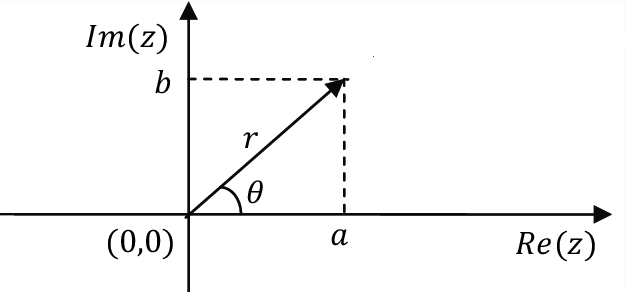
\includegraphics[width=0.7\linewidth]{Figuras/Ch15/complexo.png}}
	\begin{block}{Forma Retangular}
		$$z = a +jb$$
		\begin{itemize}
			\item $j = \sqrt{-1}$
			\item $a$: parte real de $z$
			\item $b$: parte imaginária de $z$
		\end{itemize}
	\end{block}
}

\frame{
	\frametitle{Números complexos}
	\setmyunit{2cm}
	\centering
	\begin{tikzpicture}
	\draw[->] (-0.2,0) -- (1.2,0) node[right] {$ \Re(z) $};
	\draw[->] (0,-0.2) -- (0,1) node[above] {$ \Im(z) $};
	
	\draw[dashed] (0,0.8) node[left] {$ b $} -- (1,0.8) -- (1,0) node[below] {$ a $};
	
	\node[below left] at (0,0) {$ (0,0) $};
	
	\draw[-Latex] (0,0) -- node[above left] {$ r $} (1,0.8);
	\coordinate (O) at (0,0);
	\coordinate (A) at (1,0);
	\coordinate (B) at (1,0.8);
	
	\pic[draw, angle radius=15pt,angle eccentricity=1,"$ \theta $" {xshift=4pt,yshift=1pt}] {angle=A--O--B};
	\end{tikzpicture}
	
%	\centerline{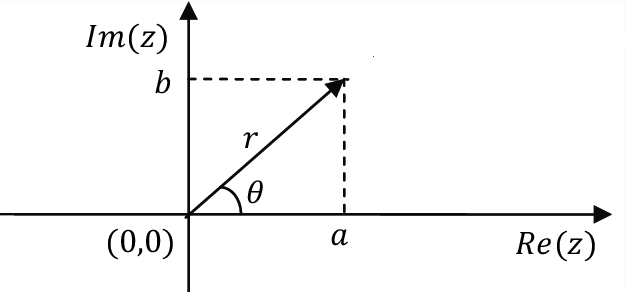
\includegraphics[width=0.7\linewidth]{Figuras/Ch15/complexo.png}}
	\begin{block}{Módulo e Fase de um número complexo}
		$$z = a +jb$$
		\begin{itemize}
			\item $r = \sqrt{a^2 + b^2}$
			\item $\theta = \arctg \Big(\dfrac{b}{a} \Big)$
		\end{itemize}
	\end{block}
}

\frame{
	\frametitle{Números complexos}
	\setmyunit{2cm}
	\centering
	\begin{tikzpicture}
	\draw[->] (-0.2,0) -- (1.2,0) node[right] {$ \Re(z) $};
	\draw[->] (0,-0.2) -- (0,1) node[above] {$ \Im(z) $};
	
	\draw[dashed] (0,0.8) node[left] {$ b $} -- (1,0.8) -- (1,0) node[below] {$ a $};
	
	\node[below left] at (0,0) {$ (0,0) $};
	
	\draw[-Latex] (0,0) -- node[above left] {$ r $} (1,0.8);
	\coordinate (O) at (0,0);
	\coordinate (A) at (1,0);
	\coordinate (B) at (1,0.8);
	
	\pic[draw, angle radius=15pt,angle eccentricity=1,"$ \theta $" {xshift=4pt,yshift=1pt}] {angle=A--O--B};
	\end{tikzpicture}
	
%	\centerline{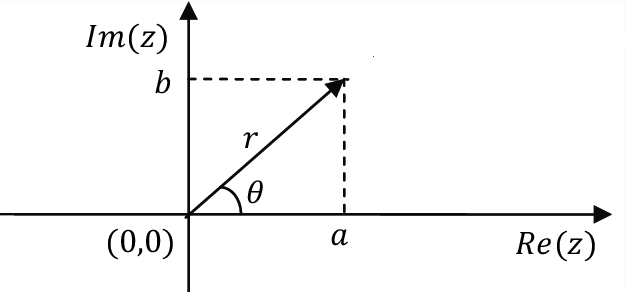
\includegraphics[width=0.7\linewidth]{Figuras/Ch15/complexo.png}}
	\begin{block}{Forma Polar}
		$$z = r \phase{\theta}$$
	\end{block}
}

\frame{
	\frametitle{Números complexos}
	\setmyunit{2cm}
	\centering
	\begin{tikzpicture}
	\draw[->] (-0.2,0) -- (1.2,0) node[right] {$ \Re(z) $};
	\draw[->] (0,-0.2) -- (0,1) node[above] {$ \Im(z) $};
	
	\draw[dashed] (0,0.8) node[left] {$ b $} -- (1,0.8) -- (1,0) node[below] {$ a $};
	
	\node[below left] at (0,0) {$ (0,0) $};
	
	\draw[-Latex] (0,0) -- node[above left] {$ r $} (1,0.8);
	\coordinate (O) at (0,0);
	\coordinate (A) at (1,0);
	\coordinate (B) at (1,0.8);
	
	\pic[draw, angle radius=15pt,angle eccentricity=1,"$ \theta $" {xshift=4pt,yshift=1pt}] {angle=A--O--B};
	\end{tikzpicture}
	
%	\centerline{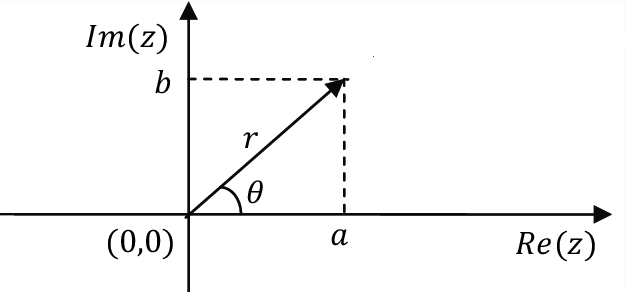
\includegraphics[width=0.5\linewidth]{Figuras/Ch15/complexo.png}}
	\begin{block}{Conversão entre as formas}
		\textbf{Retangular para Polar}
		\begin{itemize}
			\item $r = \sqrt{a^2 + b^2}$
			\item $\theta = \arctg \Big(\dfrac{b}{a} \Big)$
		\end{itemize}
		\textbf{Polar para Retangular}
		\begin{itemize}
			\item $a = r \cdot \cos \theta$
			\item $b = r \cdot \sen \theta$
		\end{itemize}
	\end{block}
}

\frame{
	\frametitle{Exemplo}
	\begin{block}{}
		01.  Converta o número complexo para a forma polar: $z = 3 + j4$ \\
		\textbf{Solução:} \\
		\begin{itemize}
			\item $r = \sqrt{a^2 + b^2} = \sqrt{3^2 + 4^2} = \sqrt{9 + 16} = \sqrt{25} = 5$
			\item $\theta = \arctg \Big(\dfrac{b}{a} \Big) = \arctg \Big(\dfrac{4}{3} \Big) = \ang{53.13}$
		\end{itemize}
		$$\text{Logo, }  z = 5 \phase{\ang{53.13}}$$
		\\
		02. Converta o número complexo para a forma retangular: $z = 10 \phase{\ang{45}}$ \\
		\textbf{Solução:} \\
		\begin{itemize}
			\item $a = r \cos \theta = 10 \cos(\ang{45}) =\num{7.07}$
			\item $b = r \sen \theta = 10 \sen(\ang{45}) =\num{7.07}$
		\end{itemize}
		$$\text{Logo, } z = \num{7.07} +j\num{7.07}$$
	\end{block}
}

\frame{
	\frametitle{Números complexos}
	\begin{block}{Propriedades e operações básicas}
		\begin{itemize}
			\item \textbf{Adição}: $z_1 + z_2 = (a_1 + a_2) + j(b_1 + b_2)$ \vspace{0.2cm}
			\item \textbf{Subtração}: $z_1 - z_2 = (a_1 - a_2) + j(b_1 - b_2)$ \vspace{0.2cm}
			\item \textbf{Multiplicação}: $z_1 \times z_2 = r_1 \times r_2 \phase{\theta_1 + \theta_2}$ \vspace{0.2cm}
			\item \textbf{Divisão}: $\dfrac{z_1}{z_2} = \dfrac{r_1}{r_2} \phase{\theta_1 - \theta_2}$ \vspace{0.2cm}
			\item \textbf{Inverso}: $\dfrac{1}{z} = \dfrac{1}{r} \phase{-\theta}$ \vspace{0.2cm}
			\item \textbf{Raiz quadrada}: $\sqrt{z} = \sqrt{r} \phase{\dfrac{\theta}{2}}$ \vspace{0.3cm}
			\item \textbf{Conjugado complexo}: $\bar{z}=z^* = a - jb = r\phase{-\theta}$
		\end{itemize}
	\end{block}
}

\frame{
	\frametitle{Exemplo}
	\begin{block}{}
		01.  Calcule o número complexo: $z = \sqrt{40 \phase{\ang{50}} + 20 \phase{\ang{-30}}}$
		
		\textbf{Solução:}
		\begin{gather*}
			40 \phase{\ang{50}} = 40 (\cos (\ang{50}) + j \sen (\ang{50}) = \num{25,71} + j\num{30,64}\\[0.25cm]
			20 \phase{\ang{-30}} = 20 (\cos (\ang{-30}) + j \sen (\ang{-30}) = \num{17,32} - j10\\[0.25cm]
			\num{25,71} + j\num{30,64} + \num{17,32} - j10 = \num{43,03} + j \num{20,64}\\[0.25cm]
			r = \sqrt{a^2 + b^2} = \sqrt{\num{43,03}^2 + \num{20,64}^2} = \num{47,42}\\[0.25cm]
			\theta = \arctg \Big(\dfrac{b}{a} \Big) = \arctg \Big(\dfrac{\num{20,64}}{\num{43,03}} \Big) = \ang{25,63}
		\end{gather*}
		
		Logo,
		$$ \sqrt{z} = \sqrt{r} \phase{\dfrac{\theta}{2}} = \sqrt{\num{47,42}} \phase{\dfrac{\ang{25,63}}{2}} = \num{6,91} \phase{\ang{12,81}}$$ \smallskip
	\end{block}
}

\frame{
	\frametitle{Análise fasorial em circuitos de C.A.}
	\begin{block}{Representação fasorial para tensão e corrente}
		A representação fasorial para tensão e corrente é feita a partir da representação temporal na forma de \textbf{cosseno}.
		\begin{itemize}
			\item Dada a cossenoide $v(t) = V_m \cos(\omega t + \theta)$, \\
			      $$\vec{V} = V_m \phase{\theta} \text{ é a representação fasorial da cossenoide } v(t)$$
		\end{itemize}
		\vspace{1cm}
		\textbf{A análise de fasores se aplica apenas quando a frequência é constante e na manipulação de dois ou mais sinais senoidais com a mesma frequência.}
	\end{block}
}

\frame{
	\frametitle{Análise fasorial em circuitos de C.A.}
	\begin{block}{Importante}
		Para representar o fasor de uma função seno, é necessário expressá-la, antes, através da função cosseno.
		
		\begin{itemize}
			\item $\sen(\omega t) = \cos(\omega t - \ang{90})$
			\item $\cos(\omega t) = \cos(\omega t + \ang{90})$
			\item $-\sen A = \cos(A + \ang{90})$
			\item $-\cos A = \cos(A \pm \ang{180})$
		\end{itemize}
	\end{block}
}

\frame{
	\frametitle{Exemplo}
	\begin{block}{}
		01. Transforme a seguinte senoide em fasor: $i(t) = 6 \cos(50t - \ang{40})$ \\ \vspace{0.2cm}
		\textbf{Solução:} \\ \vspace{0.2cm}
		$\vec{I} = 6 \phase{\ang{-40}}$

		\vspace{0.7cm}

		02. Transforme a seguinte senoide em fasor: $ v(t) = -4 \sen(30t + \ang{50})$ \\ \vspace{0.2cm}
		\textbf{Solução:} \\ \vspace{0.2cm}
		$v(t)= -4 \sen(30t + \ang{50}) = 4 \cos(30t + \ang{50} + \ang{90}) = 4 \cos(30t + \ang{140}) \implies$
		
		$\vec{V}= 4 \phase{\ang{140}}$

		\vspace{0.7cm}

		03. Determine a senoide representada pelo fasor $\vec{V} = -25 \phase{\ang{40}}$ \\ \vspace{0.2cm}
		\textbf{Solução:} \\ \vspace{0.2cm}
		$v(t) = 25 \cos(\omega t - \ang{140}) \text{ ou } v(t) = 25 \cos(\omega t + \ang{220})$
	\end{block}
}

\frame{
	\frametitle{Relações entre fasores para elementos de circuitos}
	\begin{block}{Resistor}
		\begin{itemize}
			\item $i(t) = I_m \cos(\omega t + \theta)$
			\item $v(t) = R\cdot i(t) = R \cdot I_m \cos(\omega t + \theta)$
		\end{itemize}
		\vspace{0.5cm}
		\textbf{No domínio da frequência (fasores):}
		\begin{itemize}
			\item $\vec{V} = R\cdot I_m \phase{\theta}$
			\item $\vec{V} = R\cdot \vec{I}$
		\end{itemize}
		\vspace{0.5cm}
		\textbf{A corrente no resistor está em fase com a tensão.}
	\end{block}
}

\frame{
	\frametitle{Relações entre fasores para elementos de circuitos}
	\centerline{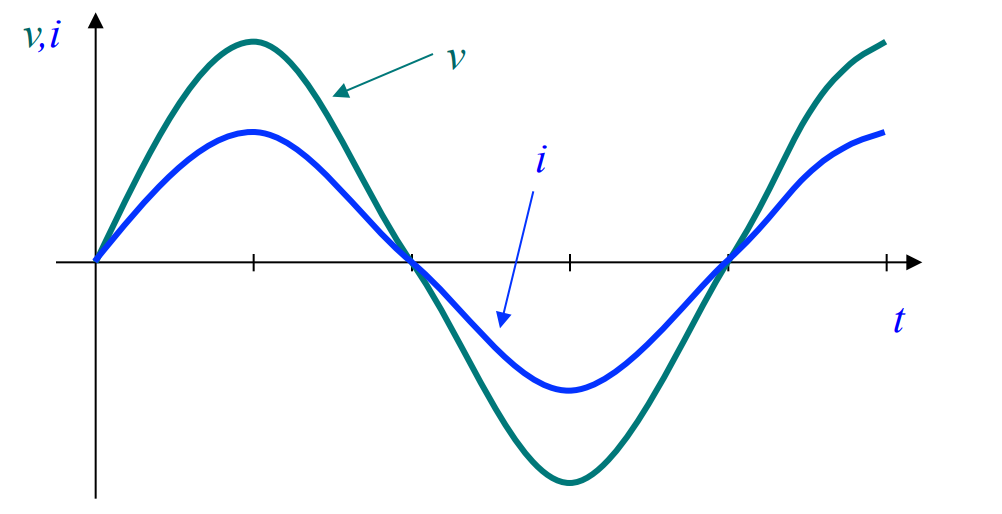
\includegraphics[width=0.5\linewidth]{Figuras/Ch15/rfasores.PNG}}
	\begin{block}{Resistor - Exemplo}
		Para $R = 5 \si{\ohm}$ e $v(t) = 10 \cos(100t + \ang{30})$, determine $\vec{I}$ e $i(t)$.
		\begin{gather*}
			\vec{V} = 10 \phase{\ang{30}}\\
			\vec{I} = \dfrac{V}{R} = \dfrac{10 \phase{\ang{30}}}{5} = 2 \phase{\ang{30}}
		\end{gather*}
		No domínio do tempo:
		$$i(t) = 2 \cos(100t + \ang{30})$$
	\end{block}
}

\frame{
	\frametitle{Relações entre fasores para elementos de circuitos}
	\begin{block}{Capacitor}
		\begin{itemize}
			\item $i(t) = I_m \cos(\omega t + \theta)$
			\item $v(t) = \dfrac{1}{\omega C} \cdot i(t) = \dfrac{1}{\omega C} \cdot I_m \cos(\omega t + \theta - \ang{90})$
		\end{itemize}
		\vspace{0.5cm}
		\textbf{No domínio da frequência (fasores):}
		\begin{itemize}
			\item $\vec{V} = \dfrac{1}{\omega C} \cdot I_m \phase{\theta - \ang{90}}$
			\item $\vec{V} = \dfrac{\vec{I}}{j \omega C}$
		\end{itemize}
		\vspace{0.5cm}
		\textbf{A corrente no capacitor
			está adiantada da tensão em \ang{90}.}
	\end{block}
}

\frame{
	\frametitle{Relações entre fasores para elementos de circuitos}
	\centerline{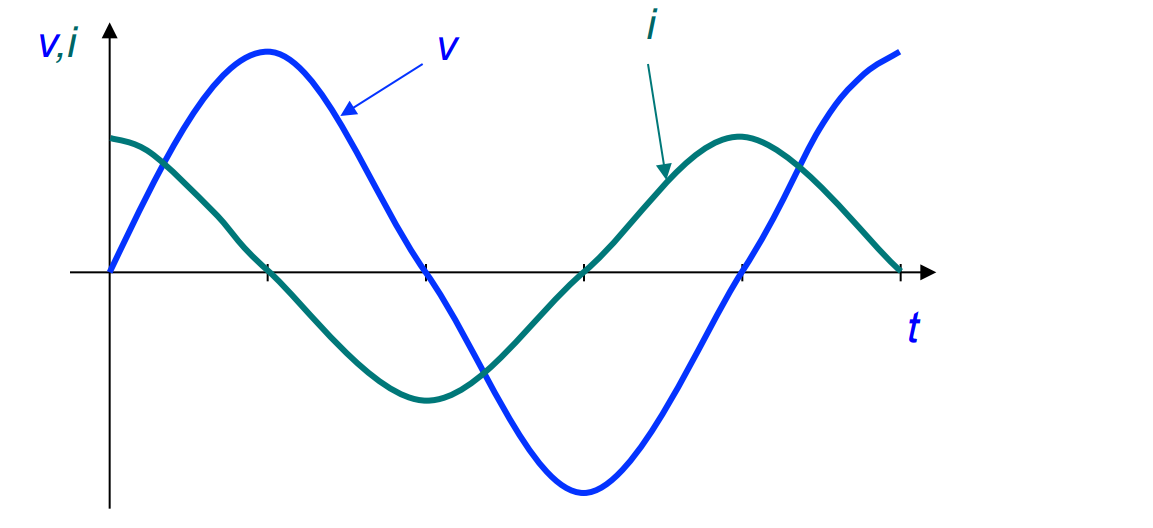
\includegraphics[width=0.5\linewidth]{Figuras/Ch15/cfasores.PNG}}
	\begin{block}{Capacitor - Exemplo}
		Para $C = \SI{1}{\micro\farad}$ e $v(t) = 10 \cos(100t + \ang{30})$, determine $\vec{I}$ e $i(t)$.
		\vspace{0.2cm}
		$$\vec{V} = 10 \phase{\ang{30}}$$
		$$\vec{I} = j \omega C \vec{V} = 100j \cdot \num{1e-6} \cdot 10 \phase{\ang{30}} = 100 \phase{\ang{90}} \cdot \num{1e-6}\cdot 10 \phase{\ang{30}} = \num{0.001}\phase{\ang{120}}$$
		No domínio do tempo:
		$$i(t) = \num{0,001} \cos(100t + \ang{120})$$
	\end{block}
}

\frame{
	\frametitle{Relações entre fasores para elementos de circuitos}
	\begin{block}{Indutor}
		\begin{itemize}
			\item $i(t) = I_m \cos(\omega t + \theta)$
			\item $v(t) = \omega L \cdot i(t) = \omega L I_m \cos(\omega t + \theta + \ang{90})$
		\end{itemize}
		\vspace{0.5cm}
		\textbf{No domínio da frequência (fasores):}
		\begin{itemize}
			\item $\vec{V} = \omega L \cdot I_m \phase{\theta + \ang{90}}$
			\item $\vec{V} = j \omega L \cdot \vec{I}$
		\end{itemize}
		\vspace{0.5cm}
		\textbf{A corrente no indutor está atrasada da tensão em $\ang{90}$.}
	\end{block}
}

\frame{
	\frametitle{Relações entre fasores para elementos de circuitos}
	\centerline{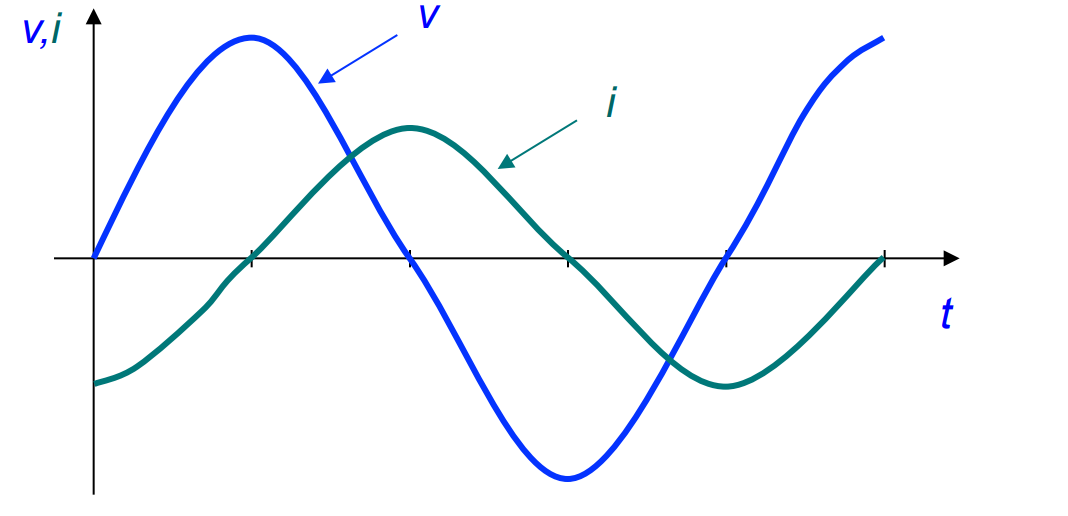
\includegraphics[width=0.5\linewidth]{Figuras/Ch15/ifasores.PNG}}
	\begin{block}{Indutor - Exemplo}
		Para $L = \SI{1}{\henry}$ e $v(t) = 10 \cos(100t + \ang{30})$, determine $\vec{I}$ e $i(t)$. \vspace{0.2cm}
		$$\vec{V} = 10 \phase{\ang{30}}$$
		$$\vec{I} = \dfrac{\vec{V}}{j \omega L} = \dfrac{10 \phase{\ang{30}}}{100j \cdot 1} = \dfrac{10 \phase{\ang{30}}}{100 \phase{\ang{90}}} = \num{0,1} \phase{\ang{-60}}$$
		No domínio do tempo:
		$$i(t) = \num{0,1} \cos(100t -\ang{60})$$
	\end{block}
}

\frame{
	\frametitle{Resumo}
	\centering
	\setmyunit{1.5cm}
	\begin{tikzpicture}
		\draw (0,0) rectangle (0.1,-0.1) node[pos=0.5] {$ \cdot $};
		\draw (0,0) rectangle (0.1,0.1) node[pos=0.5] {$ \cdot $};
		\draw[->] (-0.2,0) -- (1.2,0) node[right] {$ \Re(z) $};
		\draw[->] (0,-1.2) -- (0,1.2) node[above] {$ \Im(z) $};
		
		\draw[-Latex,blue] (0,0) -- (0,1) node[right] {$ X_L\phase{\ang{90}} $};
		\draw[-Latex,blue] (0,0) -- (1,0) node[below] {$ R\phase{\ang{0}} $};
		\draw[-Latex,blue] (0,0) -- (0,-1) node[left] {$ X_C\phase{\ang{-90}} $};
	\end{tikzpicture}
	
%	\centerline{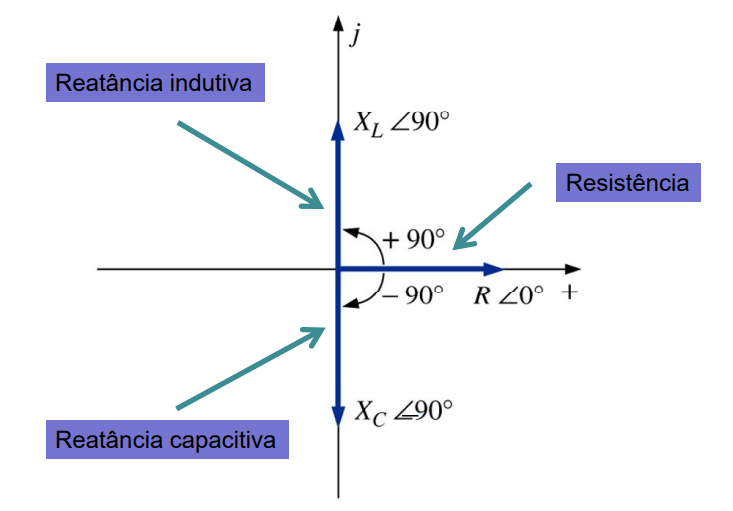
\includegraphics[width=0.6\linewidth]{Figuras/Ch15/resumo.PNG}}
	\begin{block}{Em resumo...}
		\begin{itemize}
			\item Ao encontrar um \textbf{resistor}: substitua por $R$
			\item Ao encontrar um \textbf{capacitor}: substitua por $-jX_C$
			\item Ao encontrar um \textbf{indutor}: substitua por $jX_L$
		\end{itemize}
	\end{block}
}

\section*{Exercícios}

\frame{
	\frametitle{Exercícios}
	\begin{block}{}
		01. Determinar $i$ no circuito a seguir.
	\end{block}

	\setmyunit{2cm}
	\centering
	\begin{circuitikz}
		\draw (0,0) to[sV, l_=$ v(t) \, {=} \, 5 \cos(3t) $] ++(0,-2) -- ++(1,0)
		to[L=1<\henry>,*-] ++(0,1)
		to[R=3<\ohm>,-*] ++(0,1)
		to[R=1<\ohm>, i<_=$ i_1 $] ++(-1,0)
		++(1,0) to[short,i=$ i $] ++(1,0)
		to[C,a=\SI{1/9}{\farad}] ++(0,-2) -- ++(-1,0);
		
	\end{circuitikz}
%	\centerline{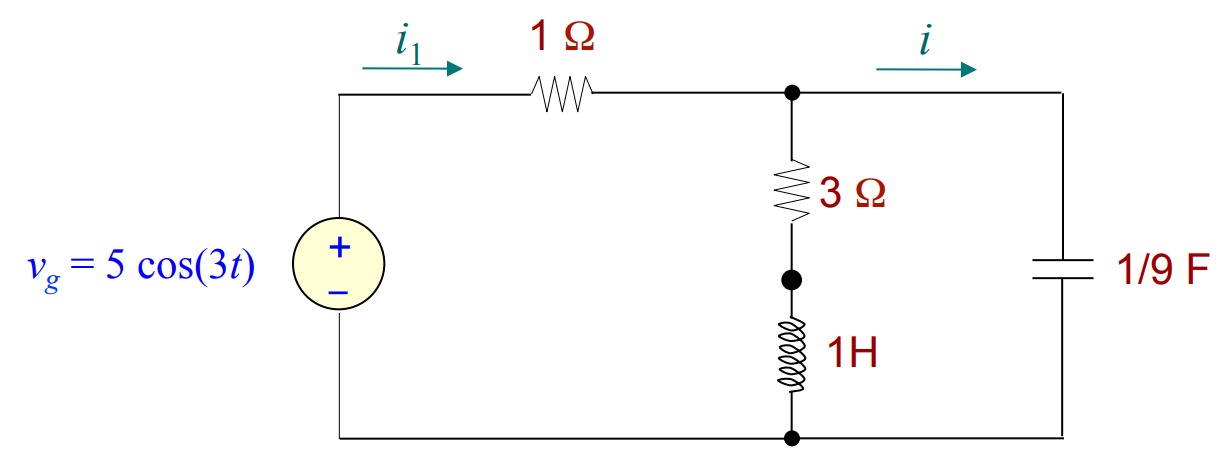
\includegraphics[width=0.9\linewidth]{Figuras/Ch15/exemplofasores.PNG}}
}


\section*{Referências}

\frame{
	\frametitle{Referências e Exercícios Complementares}
	\begin{itemize}
		\item ALEXANDRE, Charles K.; SADIKU, Matthew N. O. Fundamentos de Circuitos Elétricos. 5. ed. Porto Alegre: AMGH, 2013.
	\end{itemize}
	%\centering{\alert{Página 36 - \textbf{1.6.1 até 1.6.5, 1.6.17 até 1.6.19}}} \\
	\centering{\alert{Lista de exercícios 15}}
}